\documentclass[FyPI.tex]{subfiles}
\newcommand*\interior[1]{#1^{\mathsf{o}}}
\begin{document}

\chapter{Fractales. Introducción.}
\section{Apuñalar a esos profesores que no dan apuntes}
No existe una definición aceptada de lo que es un objeto fractal, aunque se acepta comúnmente que los fractales deben tener ciertas características.
\begin{enumerate}
\item Poseen \textbf{autosemjanza} o \textbf{autosimilitud}, ya sea general o por zonas.
\item Tienen una \textbf{dimensión fractal}, que será mayor o igual que su dimensión topológica.
\item Son conjuntos, en cierto sentido, \textbf{irregulares}.
\end{enumerate}
\section{Conjunto de Cantor}
Consideremos el intervalo $[0,1]$. Realizamos un proceso iterativo en el que dividimos el conjunto en tres partes iguales y eliminamos la parte de en medio. Aplicamos iterativamente este procedimiento a los suscesivos intervalos que se van generando. 
\begin{figure}[h!]
\centering
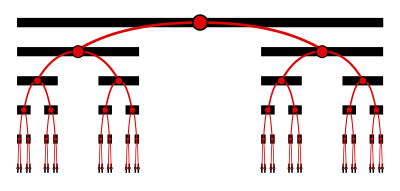
\includegraphics[scale=0.7]{prueba}
\end{figure}
Para codificar estos intervalos, vamos a notar a los intervalos de la siguiente manera. En la primera división llamamos al primer intervalo $I_0$ y al segundo $I_1$, y a su unión $C_1$. A los cuatro siguientes, $I_{00}$, $I_{01}$, $I_{10}$ e $I_{11}$, y a la unión $C_2$. Y así, sucesivamente.

El conjunto de cantor es la intersección de todos los $C_i$ y, al estar encajados, es de hecho el límite de los $C_i$. Notemos que $\forall i \geq 1$ $C_i \subset C_{i-1}$. Denotamos por $C$ el conjunto de Cantor. 
\newpage
Vamos a calcular la longitud de $C$. Notemos que
$$
m(C_i) = \left(\frac{2}{3}\right)^i \qquad \lim_{i\to\infty} m(C_i) = 0
$$
Dado que $C\subset C_i$  y la medida $m(\cdot)$ es monótona y no negativa, se tiene que $m(C)=0$.

Una vez vista su medida, pasamos a ver su cardinalidad. Recordemos que $\forall x \in [0,1]$ 
$$
x = \sum_{n=1}^\infty \frac{a_n}{3^n} \quad a_n\in \{0,1,2\}
$$
Aunque esta representación no es única, pues
$$
\frac{1}{3} = \sum_{n=2}^\infty \frac{2}{3^n}
$$
Lo que sí es cierto con respecto a esta dualidad es que cualquier $x$ que tenga un representación finita también va a tener una representación infinita. Puede probarse que
$$
C=\{0\}\cup\{x\in(0,1] \mid x = \sum_{n=1}^\infty \frac{a_n}{3^n},\text{ suma infinita, }\;a_n = 0,2,\; n \in \mathbb{N}\}
$$
Antes de continuar, tenemos que saber que en la literatura matemática es frecuente encontrar que el conjunto
$$
C=\{0,1\}^\mathbb{N} = \{f:\mathbb{N} \to \{0,1\}\} = \{(\varepsilon_1,\varepsilon_2,\dotsc)\mid \varepsilon_i \in \{0,1\}\}
$$
es denominado conjunto de Cantor. Vamos a definir una aplicación que conecte ambos conjuntos de Cantor:
$$
\phi(\varepsilon_1,\varepsilon_2,\dotsc) = \sum_{n=1}^\infty \frac{2\varepsilon_n}{3^n}
$$
Se puede probar que $\phi$ es una biyección. Además, este nuevo conjunto de cantor tiene una biyección trivial con $\R$, a saber
$$
f:\{0,1\}^\mathbb{N} \to [0,1] \qquad (\varepsilon_1,\varepsilon_2,\dotsc) \to \sum_{n=1}^{\infty} \frac{\varepsilon_n}{2^n}
$$
Por tanto, el conjunto de Cantor tiene cardinalidad infinita no numerable.

Veamos otra forma de reproducir el conjunto de Cantor. Partamos del intervalo $I=\{0,1\}$, aunque podríamos utilzar otro. Definimos las aplicaciones
\begin{align*}
T_0& : [0,1]\to [0,1] & T_1&:[0,1]\to [0,1] \\
x& \to \frac{1}{3}x & x &\to \frac{1}{3}x+\frac{2}{3}
\end{align*}
Naturalmente $T_0(I) = [0,1/3]$ y $T_1(I)=[2/3,1]$. Definimos $T(A)=T_0(A)\cup T_1(A)$. Por tanto
$$
T(C_1) = T_0(C_1)\cup T_1(C_1) = C_2, \qquad T(C_n) = C_{n+1}
$$
\section{Triángulo de Sierpinski}
 Partimos de un triángulo, en principio equilatero aunque no tiene por qué. Dividimos en cuatro triángulos iguales y desechamos el interior. Comenzando por el que corresponde a la base en el lado izquierdo numeramos en sentido contrario a las agujas del reloj $E_0$, $E_1$ y $E_2$ análogamente a como hicimos en el conjunto de Cantor. Repetimos iterativamente el proceso sobre estos triángulos. Podemos considerar los conjuntos $E_{00}$, $E_{01}$, $E_{02}$, $E_{10}$, etc. Así, denotamos
$$
S_1 = E_0 \cup E_1 \cup E_2 \qquad S_2 = \bigcup_{e_1,e_2 \in \{0,1,2\}} E_{e_1 e_2}
$$
y análogamente definimos $S_n$. Naturalmente $S_n \subset S_{n-1}$ para $n\geq 1$. Denominamos Triángulo de Sierpinski a la intersección de todos ellos. Se puede probar que el conjunto es no vacío y de cardinalidad no numerable. Se puede probar que $m(S) = 0$ como subconjunto de $\R^2$ usando que $m(S_n)=\left(\dfrac{3}{4}\right)^n$.
\begin{figure}[h!]
\centering
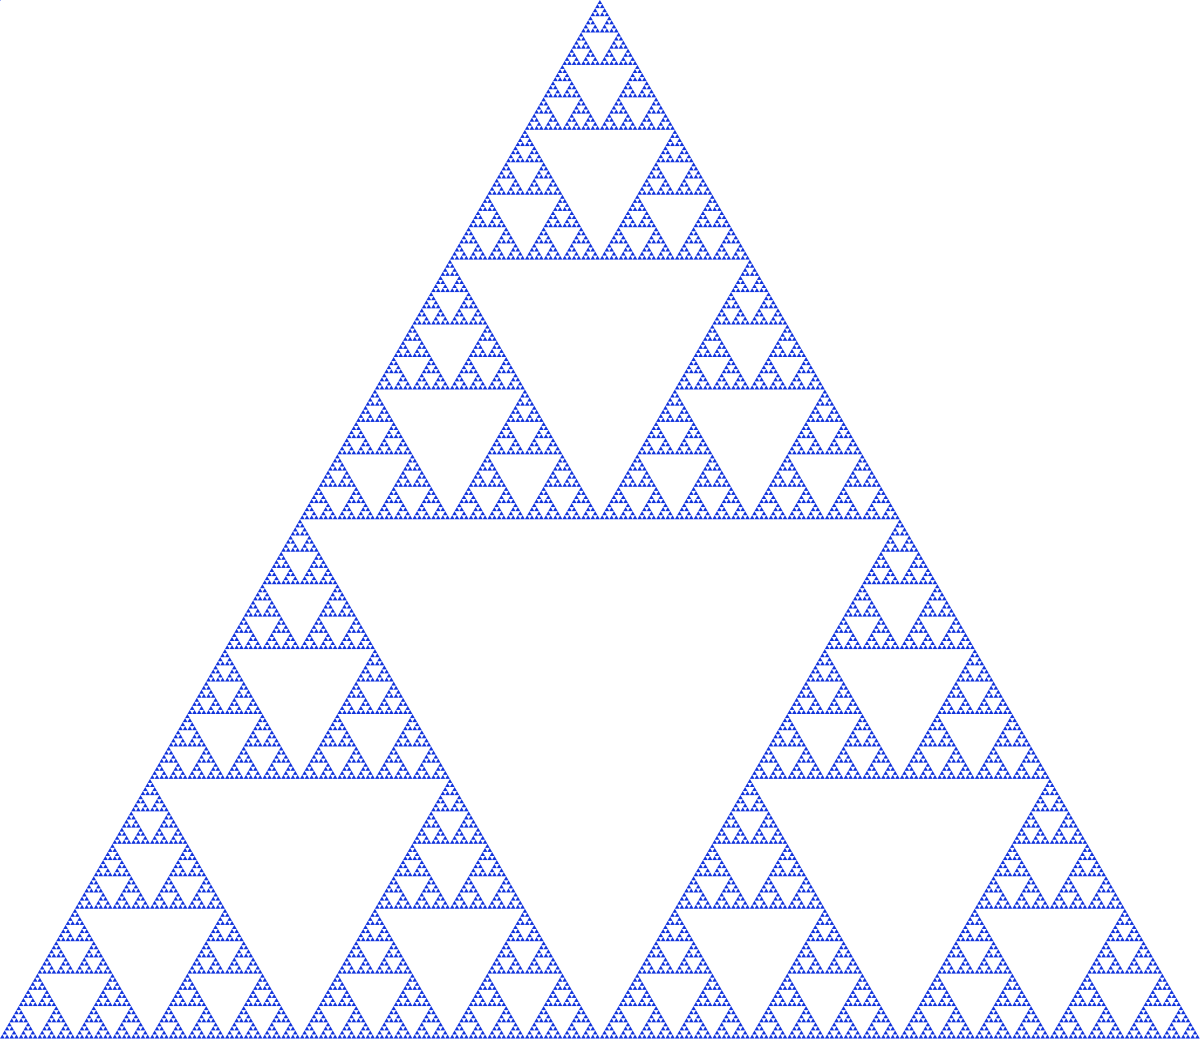
\includegraphics[scale=0.2]{sierpi}
\end{figure}

Otra forma de reproducir este conjunto es considerar $S$ el triángulo equilatero cuya base está en $[0,1]$ y está en el primer cuadrante. 
\begin{align*}
T_0 &: S\to S & T_1&:S\to S & T_2&: S\to S \\
(x,y)& \to \frac{1}{2}(x,y) & (x,y) &\to \frac{1}{2}+ (1/2,0) & (x,y) & \to \frac{1}{2} (x,y)+(1/4,\sqrt{3}/4)
\end{align*}
Si definimos $T(A) = T_0(A)\cup T_1(A)\cup T_2(A)$ entonces $T(S) = S_1$, $T(S_1) = S_2$ y, en general, $T(S_n) = S_{n+1}$.


\chapter{Sistema de funciones iteradas}
\section{Espacios métricos}
\begin{defi}
Sea $X$ un conjunto. Una \textbf{métrica} o \textbf{distancia }en $X$ es una aplicación $d: X\times X \to [0,\infty)$ que verifica
\begin{itemize}
\item Si $x=y$ si y solo si $d(x,y)=0$.
\item La aplicación es simétrica, es decir, $\forall x,y\in X$ $d(x,y)=d(y,x)$.
\item Se verifica la desigualdad triangular, es decir, $\forall x,y,z \in X$ 
$$
d(x,y)\leq d(x,z)+d(z,y)
$$
\end{itemize}
\end{defi}
\begin{defi}
Diremos que $(X,d)$ es un \textbf{espacio métrico} si $X$ es un conjunto y $d$ es una distancia en $X$.
\end{defi}
\begin{nota}
Sea $x\in X$, $\varepsilon >0$. Denotamos
$$
B(x,\varepsilon) = \{y \in X \mid d(x,y)<\varepsilon\}
$$
\end{nota}
\begin{defi}
Sea $A\subset X$. Diremos que $A$ es \textbf{abierto} si $\forall x \in A$ $\exists \varepsilon>0$ tal que $B(x,\varepsilon)\subset A$. Diremos que $A$ es \textbf{cerrado} si $A^c$ es abierto.
\end{defi}
\begin{example}
Algunos ejemplos de espacios métricos son 
\begin{itemize}
\item $(\R,|\cdot|)$, donde $d(x,y)=|x-y|$.
\item $(\R^n,d_e)$, donde $d_e = \sqrt{(x-y)'(x-y)}$.
\item $(\R^n,d_1)$, donde $d_1 = \sum_{i=1}^n |x_i-y_i|$.
\item $(\R^n,d_\infty)$, donde $d_\infty = \max_{1\leq i \leq n} |x_i-y_i|$.
\end{itemize}
\end{example}
\begin{defi}
Sea $(X,d)$ un espacio métrico y sea $A\subset X$. Definimos el \textbf{interior de $A$} y notaremos $\interior{A}$ como el conjunto
$$
\interior{A} = \{x\in A \min \exists \varepsilon >0 B(x,\varepsilon)\subset A\}
$$
Definimos además la \textbf{clausura de $A$} y notaremos $\overline{A}$ como el conjunto
$$
\overline{A} = \{ x\in X \mid \forall \varepsilon > 0 \; B(x,\varepsilon)\cap A \neq \emptyset\}
$$
\end{defi}
\begin{prop}
En las condiciones de la definición anterior, se verifica
$$
\interior{A}\subset A \subset \overline{A}
$$
\end{prop}
\begin{ejer}
En las condiciones de la definición anterior, $\interior{A}$ es el mayor abierto contenido en $A$ y $\overline{A}$ es el menor cerrado que contiene a $A$.
\end{ejer}

\begin{defi}
Sea $(X,d)$ un espacio métrico. Una \textbf{sucesión} en $X$ es una aplicación $\phi:\N\to X$. Usualmente notaremos a la sucesión $\{x_n\}_n$.
\end{defi}
\begin{defi}
Sea $\{x_n\}_n$ una sucesión en $X$ y sea $\phi:\N\to \N$ una aplicación creciente de $\{x_n\}$. Una \textbf{subsucesión} de $\{x_n\}_n$ es $\{x_{\phi(n)}\}_n$. Usualmente notaremos $\{x_{n_k}\}_k$ . 
\end{defi}
\begin{defi}
Sea $(x,d)$ un espacio métrico y $\{x_n\}_n$ una sucesión $X$ y $x\in X$. Diremos que $\{x_n\}_n$ \textbf{converge a} $x$ y notaremos 
$$
\lim_n x_n = x
$$
si se verifica
$$
\lim_n d(x_n,x) = 0
$$
\end{defi}
\begin{defi} Sea $(X,d)$ un espacio métrico $K\subset X$. Decimos que $K$ es compacto si toda sucesión $\{x_u\}\subset K$ tiene una sucesión convergente a un punto $K$.
\end{defi}
\begin{ejer}
Sea $(X,d)$ espacio métrico, entonces $A$ es cerrado si y solo sí contiene todos los puntos límites de las sucesiones contenidas en $A$.
\end{ejer}
\begin{ejer}
Sea $K$ compacto y $A\subset K$ cerrado. Entonces $A$ es compacto.
\end{ejer}
\begin{ejer}
Sea $K\subset X$ un compacto, entonces $K$ es cerrado y acotado.
\end{ejer}
\begin{theorem}[Heine] En cualquiera de los espacios métricos $(\R^n,d_e)$, $(\R^n,d_1)$ o $(\R^n,d_\infty)$ ser compacto es equivalente a ser cerrado y acotado.
\end{theorem}
\begin{defi}
Sea $\{x_n\}$ una sucesión en un espacio métrico $(X,d)$. Diremos que $\{x_n\}$ es una \textbf{sucesión Cauchy} si 
$$
\lim_{m,n}d(x_n,x_m) = 0
$$ 
Esto es, si $\forall \varepsilon >0$ $\exists n_0$ tal que $\forall n,m>n_0$ $d(x_n,x_m)<\varepsilon$.
\end{defi}
\begin{defi}
Sea $(X,d)$ un espacio métrico. Diremos $(X,d)$ es un espacio métrico completo si toda sucesión de Cauchy es convergente.
\end{defi}
\begin{theorem}
Cualquiera de los espacios métricos $(\R^n,d_e)$, $(\R^n,d_1)$ o $(\R^n,d_\infty)$  son espacios métricos completos.
\end{theorem}
\begin{lema}
Sea $(X,d)$ un espacio métrico y sea $\{x_n\} \subset X$ una sucesión. Si $d(x_n,x_{n+1})\leq a_n$ y $\sum_n a_n < \infty$ entonces $\{x_n\}$ es de Cauchy.
\end{lema}
\begin{dem}
Sea $\varepsilon >0$ y supongamos que $m>n$. Aplicando la desigualdad triangular
\begin{align*}
d(x_m,x_n) &\leq \sum_{i=n}^{m-1} d(x_{i+1},x_i)\leq \sum_{i=n}^{m-1} a_i 
\end{align*}
Como la serie es convergente, el resto de la serie tiende a $0$. Por tanto, $\exists n_0$ tal que $\forall k> n_0$ $\sum_{i=n}^\infty a_i < \varepsilon$. Por tanto, si $m,n>n_0$ tenemos que $d(x_m,x_n)<\varepsilon$ y, por tanto, el resultado.
\end{dem}
\begin{ejer}
Sea $(X,d)$ un espacio métrico y sea $F\subset X$ cerrado. entonces $(F,d)$ es un espacio métrico completo.
\end{ejer}
\begin{lema}
Sea $(X,d)$ un espacio métrico y $\{x_n\}$ una sucesión de Cauchy. Si $\{x_n\}$ tiene una sucesión convergente, entonces $\{x_n\}$ también lo es.
\end{lema}
\begin{dem}
Sea $\{x_{n_k}\}$ subsucesión convergente a $x$ de $\{x_n\}$. Basta aplicar la desigualdad triangular de la siguiente forma. Tomamos $x_{n_k}$ suficientemente cerano a $x_n$, lo cuál es posible por ser de Cauchy, y lo suficientemente cerca de $x$, de manera que 
$$
d(x_n,x) \leq d(x_n,x_{n_k}) + d(x_{n_k},x) < \varepsilon
$$
\end{dem}
\begin{defi}
Sea $(X,d)$ un espacio métrico. Diremos que $A\subset X$ es \textbf{totalmente acotado} si $\forall \varepsilon>0$ existe una cantidad finita de bolas de radio $\varepsilon$ que contiene a $A$.
\end{defi}
\begin{defi}
Sea $(X,d)$ un espacio métrico. Diremos que $K\subset X$ es relativamente compacto si toda sucesión en $K$ tiene una subsucesión convergente a un punto de $X$.
\end{defi}
\begin{lema}
Sea $(X,d)$ un espacio métrico y $K\subset X$
\begin{enumerate}
\item Si $K$ es relativamente compacto entonces $\overline{K}$ es compacto.
\item Si $K$ es compacto entonces $K$ es totalmente acotado.
\item Si $K$ es totalmente acotado entonces toda subsucesión en $K$ tiene una subsucesión de Cauchy.
\end{enumerate}
\end{lema}
\begin{dem}
\begin{enumerate}
\item[]	
\item El primer apartado es trivial.
\item Sea $\varepsilon$ que no cumpla la condición. Sea $x_1 \in K$. Naturalmente, $K\neq\subset B(x_1,\varepsilon)$. Entonces $\exists x_2$ que no está en dicha bola. $K$ no está contenida en la unión de dichas y bolas y podemos tomar un $x_3$ que no esté en ninguna. Generamos un sucesión $\{x_n\}$ tal que $\forall m,n$ $d(x_n,x_m)>\varepsilon$, lo cuál no es posible, pues ha de tener una subsucesión convergente por compacidad.
\item Sea $\{x_n\}\subset K$. Para $\varepsilon=1/2$ tenemos que la sucesión está contenida en un número finito de bolas, luego en una de ellas al menos ha de haber una cantidad infinita. Entre esos dos de estos términos la distancia entre cualesquiera de ellos es menor que $1$. Restringiendonos a estos elementos, consideramos un razonamiento análogo para $\varepsilon=1/2^2$ y así sucesivamente. Para cada $k$ tenemos un sucesión $\{x^k_n\} \subset \{x_n^{k-1}\}$ tal que $d(x_n^k,x_m^k) < 1/2^{k-1}$. Tomando la sucesión diagonal, tenemos la sucesión de Cauchy deseada.
\end{enumerate}
\end{dem}
\section{Teorema de la aplicación contractiva}
\begin{defi}
Sea $(X,d)$ un espacio métrico y sea $T:X\to X$. Diremos que $T$ es una \textbf{contracción} si $\exists 0<c<1$ tal que $d(T(x),T(y))\leq c d(x,y)$ $\forall x,y \in X$.
\end{defi}
\begin{example}
Las aplicaciones $T_0$ y $T_1$ definidas en el epígrafe del conjunto de Cantor, con respecto a $(\R,d_e)$, y $T_0,T_1,T_2$ para el triángulo de Sierpinski, con respecto a $(\R^2,d_e)$, son contractivas.
\end{example}
\begin{defi}
Sea $T:X\to X$ una aplicación. Diremos que $x \in X$ es un \textbf{punto fijo de} $T$ si $T(x)=x$. 
\end{defi}
\begin{theorem}[Banach (1922)] Sea $(X,d)$ espacio métrico completo y sea $T:X\to X$ una contracción de constante $0<c<1$. Entonces $\exists! x^*$ tal que $x^*$ es punto fijo. Además, $\forall x\in X$ la sucesión iterada $\{T^n(x)\}$ converge al punto fijo y una cota del error que cometemos es
$$
d(T^n(x),x_0) \leq \frac{c^n}{1-c}d(x,T(x))
$$
\end{theorem}
\begin{dem}
Si hubiese dos puntos fijos $x^*,y^*$, entonces
$$
d(T(x^*),T(y^*)) \leq c d(x^*,y^*) < d(x^*,y^*)
$$
Pero si $x^*$ e $y^*$ son puntos fijos, esto es una contradicción. Por tanto, a lo sumo, existe un único punto fijo. Además, sea $x\in X$, consideremos la sucesión $\{T^n(x)\}$. Veamos que es de Cauchy. Para ello, comprobamos
\begin{align*}
d(T^{n+1}(x),T^n(x)) \leq c d(T^n(x),T^{n-1}(x)) \leq c^n d(T(x),x)
\end{align*}
Como $0<c <1$, $\{c^n d(T(x),x)\}$ es convergente. Por el razonamiento anterior, tenemos que $\{T^n(x)\}$ de Cauchy y, al estar en un espacio métrico, es convergente. 

Veamos que el límite, que denotamos $x_0$ es un punto fijo. Para ello, basta tener en cuenta que si $\{T^n(x)\}\to x_0$ entonces $\{T^{n+1}(x)\}\to T(x_0)$, pero las series son exactamente la misma salvo el primer término, luego convergen al mismo límite. Luego $T(x_0)=x_0$. Por tanto, el límite es nuestro punto fijo $x^*$.

Finalmente, para obtener la cota basta usar las propiedades del punto fijo. Supongamos que $m>n$
\begin{align*}
d(T^m(x),T^n(x^*)) & = d(T^m(x),T^{m-1}(x) + \dotsc + d(T^{n+1}(x),T^n(x))\\
& \leq c^{m-1}d(x,T(x)) + \dotsc + c^n d(x,T(x)) \\
& \leq \sum_{i=n}^\infty c^i d(x,T_(x))\\
&= \frac{c^n}{1-c}d(x,T(x))
\end{align*}
\end{dem}

\section{Métrica de Hausdorff}
\begin{defi}
Dado un espacio métrico completo $(X,d)$, definimos 
$$
K(X) = \{ A\subset X\mid A\neq \emptyset, \; \text{$A$ es compacto}\}
$$
\end{defi}
\begin{nota}
Sea $A \in K(X)$ y sea $\varepsilon >0$, entonces notamos
$$
A(\varepsilon) = \{x\in X \mid \exists a\in A \; d(x,a)\leq \varepsilon\}
$$
\end{nota}
\begin{defi}
En las condiciones anteriores, definimos la distancia de Hausforff como 
\begin{gather*}d_H:K(X)\times K(X)\to [0,\infty)\\
d_H(A,B) = \inf\{\varepsilon>0,A\subset B(\varepsilon)\subset A, B\subset A(\varepsilon)\}
\end{gather*}
\end{defi}
\begin{prop} La distancia de Hausodorf es, precisamente, una distancia.
\end{prop}
\begin{dem}
\begin{itemize}
\item[]
\item Primero probaremos que $d_H(A,B) = 0 \Leftrightarrow A=B$. Naturalmente, una de las implicaciones es trivial. Supongamos que $d_H(A,B)=0$. Vamos a probar que $A\subset B$, pues la inclusión recíproca es análoga. Sea $x \in A$. Sea $\{\varepsilon_n\}$ positiva con límite $0$. Entonces, $\forall n>0$ $x \in B(\varepsilon_n)$, lueg $A\subset B(\varepsilon_n)$. Por tanto, $\forall n \in \N$ $\exists b_n \in B$ tal que $d(x,b_n) \leq \varepsilon_n$. Como $B$ es cerrado y $\{b_n\}\to x$, tenemos el resultado.
\item La simetría es trivial.
\item Para la desigualdad triangular, consideremos $A,B,C$. Sean $\varepsilon_1,\varepsilon_2$ tales que $d_H(A,C)<\varepsilon_1$ y $d_H(C,B)<\varepsilon_2$. Entonces
$$
A\subset C(\varepsilon_1) \qquad C \subset B(\varepsilon_2)
$$
Tenemos por tanto que $A \subset B(\varepsilon_1+\varepsilon_2)$.
Análogamente, podemos probar que $B\subset Az(\varepsilon_1+\varepsilon_2)$.
\end{itemize}
\end{dem}

\begin{theorem}
Si $(X,d)$ es un espacio métrico completo entonces $(K(X),d_H)$ es un espacio métrico completo.
\end{theorem}
%\begin{dem}
%Sea $\{C_n\}$ una sucesión de Cauchy en $K(X)$. Consideremos la sucesión $\varepsilon_k = 2^{-k+1}$. En particular, $\exists n_1$ tal que $\forall n,m\geq n_1$ $d_H(C_n,C_m)<1/2^2$. Podemos tomar $m=n_1$. Además, $\exists n_2 (>n_1)$ tal que $\forall m\geq 2$ $d_H(C_m,C_{n_2})<1/2^3$. En particular, $d(C_{n_2},C_{n_1})<1/2^2$. Iterando este proceso, podemos encontrar una subsucesión $n_i$ tal que
%$$
%d_H(C_{n_{i+1}},C_{n_i}) < \frac{1}{2^{i+1}}
%$$ 
%Basta probar que $\{C_k\}:= \{C_{n_k}\}$ es convergente. En particular, $\forall m \geq n$
%$$
%d_H(C_m,C_n) < \frac{1}{2^n}
%$$
%Sea
%$$
%C_0 = \bigcap_n \overline{\bigcup_{k\geq n} C_k}
%$$
%Se puede probar que 
%$$
%C_0 = \{x \in X \mid \exists \{C_{n_k}\} \subset \{C_n\}, \; \exists x_k \in C_{n_k} \mid \lim_k x_{n_k} = x \}
%$$
%Consideremos entonces $x_i \in C_i$. Entonces $d(C_{i+1},C_i)<1/2^{i+1}$ , luego $\exists x_{i+1} \ in C_{i+1}$ tal que $d(x_{i+1},x_i)<1/2^{i+1}$. Esta sucesión tiene límite, pues es de Cauchy y $(X,d)$ es espacio métrico. Naturalmente, $x \in C_0$. Por tanto, $C_0 \neq \emptyset$.

%Veamos que $C_0$ es compacto. Sea $\bigcup_{n\geq 1} C_n$. Sea $\varepsilon >0$, $\exists n_0$ tal que $1/2^{n_0} < \varepsilon/2$. Sabemos que $C_n \subset C_{n_0}(1/2^{n_0})$, pues $d_H(A,B)<\varepsilon$ si y solo si $A\buset B(\varepsilon)$ y $B\subset A(\varepsilon)$. Por 
%\end{dem}
\begin{defi} Sea $(X,d)$ un espacio métrico. Definimos un \textbf{sistema iterado de funciones} como un conjunto finito de aplicaciones contractivas $\{T_i:X\to X,\;i=1,\dotsc,m\}$. Diremos además que $F\neq \emptyset$ compacto de $X$ es \textbf{atractor} del IFS si 
$$
F_0 = \bigcup_{i_1}^m T_i(F_0)
$$

\end{defi}
\begin{lema}
Sea $(C,d)$ espacio métrico y $\{T_1,\dotsc,T_m\}$ un IFS donde cada $T_i$ tiene constante de contractividad $c_i$. Definimos
$$
T:(K(X),d_H)\to (K(X),d_H) \qquad T(A) = T_1(A)\cup \cdots \cup T_m(A)
$$
entonces $T$ esta bien definida y es una contracción con constante $c=\max_i c_i$.
\end{lema}
\begin{dem}
Claramente $T(A)$ está bien definida. Sea $A,B\in K(X)$. Entonces
$$
d = d_H(A,B) < d+ \varepsilon \Rightarrow A\subset B(d+\varepsilon)
$$
Sea $x \in T(A)$ $\exists i$ tal que $x \in T_i(A)$, luego $\exists a \ni A$ tal que $x=T_i(a)$. Como $A\subset B(d+\varepsilon)$, $\exists b \in B$ tal que $d(a,b)\leq d+\varepsilon$. Entonces
$$
d(x,T_i(b)) = d(T_i(a),T_i(b)) \leq c_{i} d(a,b) \leq c(d+\varepsilon)
$$
Por tanto, $T(A)\subset T(B)(c(d+\varepsilon))$ y $T(B)\subset T(A)(c(d+\varepsilon))$, luego
$$
d_H(T(A),T(B)) \leq c(d_H(A,B)+\varepsilon)$$
\end{dem}
\begin{theorem}
Sea $(X,d)$ un espacio métrico completo y $\{T_1,\dotsc,T_s\}$ un IFS definido en $X$. Entonces $\exists! F_0 \neq \emptyset$ compacto tal que 
$$
F_0 = T_1(F_0) \cup \cdots \cup T_s(F_0)
$$ 
$F_0$ se conoce como \textbf{atractor o fractal} asociado al IFS.

\end{theorem}
\begin{prop}
En las condiciones del teorema anterior, si existe $F \in K(X)$ tal que $T(F)\subset F$ entonces
$$
F_0  = \bigcap_n T^n (F)
$$
\end{prop}
\begin{dem}
Veamos una contención. Sea $x$ en la intersección, tomamos $\varepsilon_n$ tal que $d_H(T^n(F),F_0)<\varepsilon_n$ con $\varepsilon_n\to0$. Por tanto, $x\in T^n(F)\subset F_0(\varepsilon_n)$. Luego $\exists x_n\in F_0$ con $d(x,x_n)<\varepsilon_n$. Es decir, tenemos una sucesión $\{x_n\}\subset F_0$ tal que $x_n \to x$. Por tanto, $x\in F_0$, ya que $F_0$ es compacto (y en particular ceerrado). 
\end{dem}

\begin{defi}
Sea $T:\R^n\to\R^n$. Diremos que $T$ es una transforrmación afín si $\exists u_0 \in \R^n$ y $L:\R^n\to\R^n$ aplicación lineal tal que $T(x)=L(x)+u_0$.
\end{defi}
\begin{defi}
Diremos que una transformación afín $T(x)=Ax+u_0$ es contractiva si la matriz $A$ que constituye la aplicación lineal tiene norma matricial compatible con la que estemos utilizando en $\R^n$ menor que $1$.
\end{defi}
\begin{nota}
En cuanto a la compatibilidad de las normas matriciales en $\R^2$ tenemos: 
\begin{itemize}
\item Si utilizamos $d_1$ entonces tomamos el máximo de las $d_1$ de las columnas.
\item Si utilizamos $d_\infty$, entonces tomamos el máximo de las $d_1$ por filas.
\item Si utilizamos $d_2$ entonces tomamos el mayor autovalor de $A^tA$.
\end{itemize}
\end{nota}
\begin{defi}
Sea $(X,d)$ un espacio métrico y $T:X\to X$. Diremos que $T$ es una similitud si $d(x,y)=c d(x,y)$.
\end{defi}
\begin{defi}
Sea $\{T_1,\dotsc,T_n\}$ un IFS donde cada $T_i$ es una similitud de constante $c_i$. Se denomina dimensión de similitud del fractal asociado a la única solución de la ecuación
$$
\sum_{i=1}^n c^S_i = 1
$$

\end{defi}
\begin{nota}
La dimensión de similitud está bien definida.
\end{nota}
\begin{example}
El conjunto de Cantor tiene dimensión $\log_3 2$, el triángulo de Sierpinski $\log_2 3$, la curva de Koch $\log 4_3$. 
\end{example}

\begin{ejercico}
Crear un sistema iterado de funciones en $\R^2$. Tomar $A\sbuset \R^2$ no vacío compacto y dibujar las iteradas del conjunto $A$ por el IFS. Aproximar el fractal obtenido como punto fijo del IFS. En caso de ser similitudes, calcular la dimensión de similaridad.
\end{document}
